%!TEX root = ../dissertation.tex
%\begin{savequote}[75mm]
%\qauthor{Quoteauthor Lastname}
%\end{savequote}

%% Set up problem
\begin{figure*}[t]
\begin{center}
{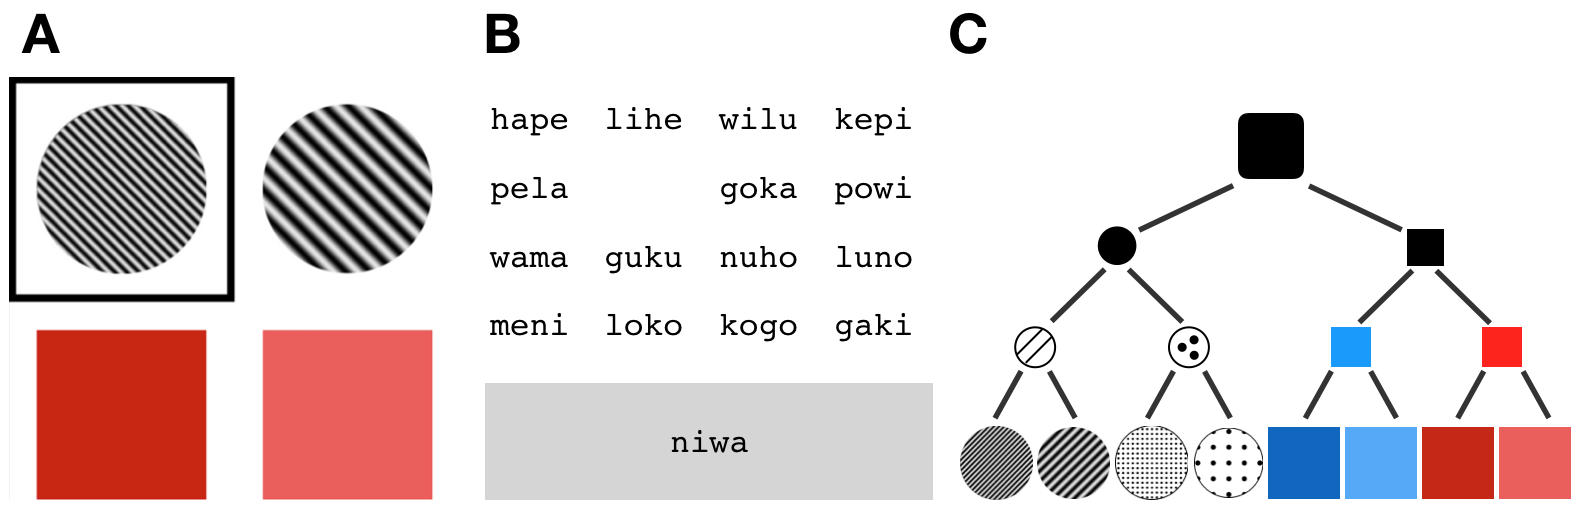
\includegraphics[scale=.63]{./figures/Sec2-design.png}}
{\caption{{\emph{Domain for context-sensitivity.} (A) Example of \emph{fine} context where one of the distractors belongs to the same fine-grained branch of the hierarchy as the target (i.e.\ another striped circle), so any abstract label would be insufficient to disambiguate them. The target is highlighted for the speaker with a black square. (B) Drag-and-drop chat box interface, where the label ``niwa'' has been selected. (C) Hierarchical organization of stimuli.\label{fig:context_design}}}}
\vspace{-2ex}
\end{center}
\end{figure*}

In the previous two sections, we examined a mechanism for rapid, partner-specific learning that allows agents to form stable but arbitrary \emph{ad hoc} conventions with partners and gradually generalize them to their entire community. 
The final phenomenon we consider is the way that \emph{ad hoc} conventions are shaped by the communicative context in which they form.
This phenomenon is most immediately motivated by recent behavioral results finding that more informative words in the local context are significantly more likely to become conventionalized as labels \cite{hawkins2020characterizing}.

However, our broader theoretical aim is to suggest that \emph{diachronic} patterns in the long-term evolution of a community's lexical conventions, as highlighted by the Optimal Semantic Expressivity (OSE) hypothesis \cite{frankblogpost}, may be explained as a result of the \emph{synchronic} processes at play in individual dyads' \emph{ad hoc} coordination on meaning.
For example, while most English speakers have the basic-level word ``tree'' in their lexicon, along with a handful of subordinate-level words like ``maple'' or ``fir,'' we typically do not have labels exclusively referring to each individual tree in our yards.
%If we need to refer to a specific tree, we instead create a referring expression \emph{on the fly} (e.g. ``the one with the bright red leaves close to the street'').
Meanwhile, we \emph{do} often have conventionalized labels (i.e. proper nouns) for individual people and places that we regularly encounter in our daily lives. \ks{If you want to be cute: there are some very famous trees that have their own names - the Fortingall Yew is my favourite, there's also that huge redwood in the US, General Sherman or whatever.}

%What determines the extension of different conventions?
As a first step toward explaining these diachronic patterns, we aim to establish in this section that our model allows a dyad's \emph{ad hoc} conventions to be shaped by context over short timescales.
That is, when the environment imposes a communicative need to refer to particular \emph{ad hoc} concepts (like a particular tree), communicative partners are able to coordinate on efficient lexical conventions for successfully doing so\footnote{By induction, the hierarchical generalization mechanisms evaluated in the previous section then provide the mechanism by which these \emph{ad hoc} conventions become adopted by a larger community over longer time scales. Many \emph{ad hoc} conventions may simply never generalize to the full language community because the contexts where they are needed are uncommon.}.
%When a particular partner uses a label to refer to an object in a context, we can infer that they do not believe it applies to the distractors as well; otherwise, they would have known it would be confusing and chosen a different label.
First, we show that context-sensitivity naturally emerges from our model, as a downstream consequence of recursive pragmatic reasoning.
We then empirically evaluate this account by manipulating the context in an artificial-language repeated reference game, allowing us to observe the emergence of \emph{ad hoc} conventions in the absence of global priors.
%This experiment manipulates the context of distractors in a repeated reference game where participants must interactively coordinate on an artificial language from scratch. 
In both the empirical data and our model simulations, we find that conventions come to reflect the distinctions that are functionally relevant for communicative success and that pragmatic reasoning is needed for these effects to arise. 
\ks{Again, I think you need to cite the Winters et al 2018 paper somewhere here - I don't think it undermines the novelty of what you are doing and it doesn't include a model, plus it's not well-suited to modelling because the signal space was entirely open-ended.}

\subsection{Model predictions}

To evaluate the impact of context on convention formation, we require a different task than we used in the previous sections.
Those tasks, like most reference games in the literature on convention formation, used a discrete set of unrelated objects in a fixed context, $\{o_1, \dots, o_k\}$. 
In real referential contexts, however, targets are embedded in larger conceptual taxonomies, where some objects are more similar than others \cite{bruner1956study,collins1969retrieval,XuTenenbaum07_WordLearningBayesian}.
Second, contexts constantly change over the coarse of an interaction: different subsets of objects are in context at different times.

To satisfy the first desideratum, we consider a space of eight objects embedded in a three-level stimulus hierarchy with shape at the top-most level, color/texture at the intermediate levels, and frequency/intensity at the finest levels (see Fig.~\ref{fig:context_design}). 
We then populate the space of possible utterance meanings $P(\phi)$ with 8 meanings at the sub-ordinate level (one for each individual object, e.g. $\phi(u) =$ ``light blue square''), 4 meanings at the basic-level (e.g. $\phi(u) =$ ``blue square''), 2 meanings at the super-ordinate level (e.g. $\phi(u) =$ ``square''), and 1 exhaustive meaning ($\phi(u) =$ ``everything''). %, and 1 ``null'' meaning, which does not apply to any of the objects.
We populate the utterance space with 8 single-word labels. 

To satisfy the second desideratum, we only displayed four of the eight objects in the context on a given trial.
Distractors could differ from the target at various level of the hierarchy, creating different types of contexts defined by the finest distinction that had to be drawn. 
In the \emph{fine} condition, we ensure that there is always a subordinate distractor (e.g. Fig.~\ref{fig:context_design}A), while in the \emph{coarse} condition, there are only basic-level distractors (e.g. a blue square when the target is a red square) \ks{I confess I still get confused about fine vs coarse - might help to give another example in the figure and also explain the intuitions about what lexical item meanings you expect to get in the two conditions?}.
We constructed the trial sequence identically for the two conditions: there are 12 blocks, where all 8 objects appeared as the target once per block (in a randomized order ensuring that no target appeared more than once in a row).
We randomly sampled the other three distractors on each trial according to the constraints of the condition.
As before, the agents swap roles on each trial, and we run 75 distinct trajectories with parameter settings of $w_L=5, w_S=10$ and memory discounting parameter of $\beta = 0.8$.% (see Model comparison below for a more thorough evaluation of these parameters).

\paragraph{Partners successfully learn to communicate}

\begin{figure}[t]
\begin{center}
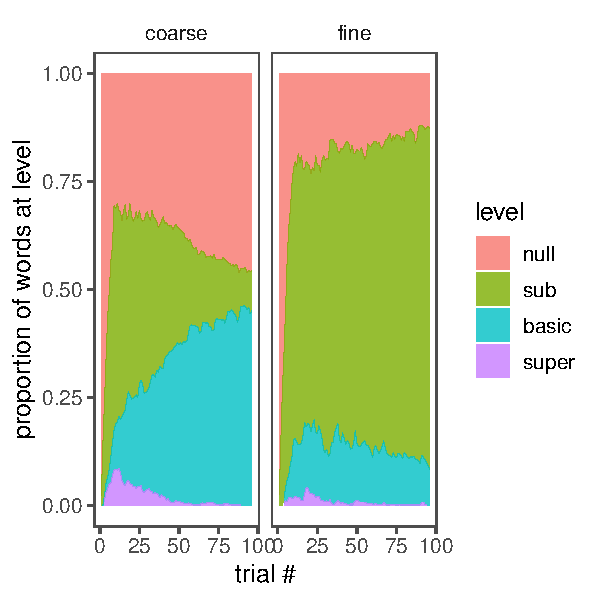
\includegraphics[scale=0.9]{evolution.pdf}
\caption{\emph{Dynamics of lexical beliefs over time in Simulation 2.1.} Regions represent the average proportion of words at each level of abstraction in an agent's beliefs about the lexicon. In the coarse condition, agents initially assume subordinate terms but gradually abstract away to a smaller number of basic-level terms; in the fine condition, however, agents become more confident of subordinate terms.}
\label{fig:evolution}
\end{center}
\end{figure}

First, we compare the model's learning curves across context conditions (Fig. \ref{fig:sec2Results}C). 
We focus on the \emph{coarse} and \emph{fine} conditions for simplicity, since this single comparison captures the core phenomena of interest.
In a mixed-effects logic regression, we find that communicative accuracy steadily improves over time across conditions, $b=0.72, z = 16.9, p<0.001$.
However, we also find a significant interaction with condition: the rate of improvement is significantly higher in the coarse condition than the fine condition, $b=-0.49, z=9.3, p <0.001$. 

\paragraph{Lexical conventions are shaped by context}

Next, we examine the effective vocabulary sizes used by speakers in each condition as a coarse marker of context sensitivity. 
We operationalized this measure by counting the total number of unique words produced within each repetition block.
Because all eight objects appeared as the target once in each block, this measure takes a maximum value of 8, in the case where a different word was used for every object, and a minimum value of 1, in the case where the same word was used for every object.
In an identical mixed-effects model, we find an overall main effect of condition, with agents in the fine condition using significantly fewer words across all repetition blocks ($m = 4.7$ in \emph{coarse}, $m=6.5$ in \emph{fine,} $t = 4.5, p < 0.001$).
However, we also found a significant interaction: the effective vocabulary size gradually increased over time in the fine condition, while it stayed roughly constant in in the coarse condition, $b = 0.18, t = 8.1, p < 0.001$, see Fig.~\ref{fig:sec2Results}D.

Finally, we examine more closely the emergence of terms at different levels of abstraction.
We have access not only to the signalling behavior of our simulated agents, but also their internal \emph{beliefs} about their partner's lexicon, which allows us to directly examine the evolution of these beliefs from the beginning of the interaction.
%So we can not only query these beliefs at the very \emph{end} of the game, as we did in our empirical post-test \ks{order messed up here, you haven't introduced the experiment yet}, we can also directly examine the evolution of these beliefs from the beginning of the interaction.
At each time point in each game, we take the single meaning with highest probability for each word.
In Fig. \ref{fig:evolution}, we show the proportion of words with meanings at each level of abstraction, collapsing across all games in each condition.

Qualitatively, we observe that agents begin with assumptions of `null' meanings \todo{I didn't follow the stuff about null meanings at all} due to their simplicity prior but quickly begin assigning meanings based on their partner's usage.
In both conditions, basic-level meanings and simpler subordinate-meanings \ks{I think this relates to my failure to grasp why lots of specific meanings is simple, but I was surprised to see this described as the simpler system} are equally consistent with the initial data, and agents prefer simpler meanings.
After the first repetition block, however, agents in the coarse condition begin pruning out some of the subordinate-level terms and become increasingly confident of basic-level meanings.
Agents in the fine condition become even more confident of subordinate level meanings.
Eventually, by the \emph{final} trial, the proportion of basic-level vs. subordinate-level terms is significantly different across the coarse and fine conditions.
Only 9\% of words had subordinate-level meanings (green) in the coarse condition, compared with 79\% in the fine condition, $\chi^2(1) = 436, p < 0.001$.
At the same time, 45\% of words had basic-level meanings (blue) in the coarse condition, compared with only 8\% in the fine condition, $\chi^2(1) = 136, p < 0.001$.
The remaining words in each condition were assigned the `null` meaning (red), consistent with an overall smaller effective vocabulary size in the coarse condition.
The diverging conventions across contexts are driven by Gricean expectations: because the speaker is assumed to be informative, only lexicons distinguishing between subordinate level objects can explain the speaker's behavior in the \emph{fine} condition.

\subsection{Experimental methods}

In this section, we evaluate our model's qualitative predictions about the effect of context on convention formation using an interactive behavioral experiment closely matched to our simulations.
We use a between-subjects design where pairs of participants are assigned to different communicative contexts and test the extent to which they converge on meaningfully different conventions.

\subsubsection{Participants}

We recruited 278 participants from Amazon Mechanical Turk to play an interactive, multi-player game using the framework described in \citeA{Hawkins15_RealTimeWebExperiments}\footnote{Planned sample sizes, exclusion criteria, and behavioral analysis plan were pre-registered at \url{https://osf.io/2hkjc/}. All statistical tests in mixed-effects models reported in this section use degrees of freedom based on the Satterthwaite approximation \cite{luke2017evaluating}.}.

\subsubsection{Procedure \& Stimuli}
Participants were paired over the web and placed in a shared environment containing an array of objects (Fig.\ \ref{fig:context_design}A) and a `chatbox' to choose utterances from a fixed vocabulary by clicking-and-dragging (Fig.\ \ref{fig:context_design}B). On each trial, one player (the `speaker') was privately shown a highlighted target object and allowed to send a single word to communicate the identity of this object to their partner (the `listener'), who subsequently made a selection from the array. Players were given full feedback, swapped roles each trial, and both received bonus payment for each correct response.

%The objects that served as referents were designed to cluster in a fixed three-level hierarchy with shape at the top-most level, color/texture at the intermediate levels, and frequency/intensity at the finest levels (see Fig.\ \ref{fig:context_design}C). Each communicative context contained four objects. Distractors could differ from the target at various level of the hierarchy, creating different types of contexts defined by the finest distinction that had to be drawn. 
%On \emph{fine} trials, the closest distractor belonged to the same fine-grained subordinate category (e.g.\ another striped circle; see Fig.\ \ref{fig:context_design}A).
%On \emph{coarse} trials, the closest distractor belonged to a coarser level of the conceptual hierarchy (e.g.\ dotted circle instead of striped circle).\footnote{Even coarser trials with super-ordinate distractors (e.g.\ a circle target among three square distractors) were logically possible but would have introduced several experimental confounds; we opted to leave these trial types out of our design and conduct the minimal manipulation.} 
We randomly generated distinct arrays of 16 utterances for each pair of participants (more than our model, which was restricted by computational complexity).
These utterances were created by stringing together consonant-vowel pairs into pronounceable 2-syllable words to reduce the cognitive load of remembering previous labels (see Fig.\ \ref{fig:context_design}B)
These arrays were held constant across trials.

%Critically, we manipulated the statistics of the context in a between-subjects design to test the context-sensitivity of conventions. 
%In the \emph{fine} condition, all targets appeared in fine contexts; in the \emph{coarse} condition, all targets appeared in coarse contexts.
To match our model as closely as possible, pairs were assigned one of the same sequences of trials that we constructed for our simulations. 
In addition to behavioral responses collected over the course of the game, we designed a post-test to explicitly probe players' final lexica. For all sixteen words, we asked players to select all objects that a word can refer to (if any), and for each object, we asked players to select all words that can refer to it (if any). 
This bidirectional measure allowed us to check the internal validity of the lexica reported.
For comparison, we also added a \emph{mixed} condition \ks{don't you need to justify why you aren't modelling the mixed condition?}, where half of the targets appeared in \emph{fine} contexts with subordinate distractors and the other half appeared in \emph{coarse} contexts.
Pairs were randomly assigned to one of three different conditions, yielding $n=36$ dyads in the \emph{coarse} condition, $n=38$ in the \emph{fine} condition, and $n=53$ in the \emph{mixed} condition after excluding participants who disconnected before completion.

%\begin{figure}[t]
%\begin{center}
%{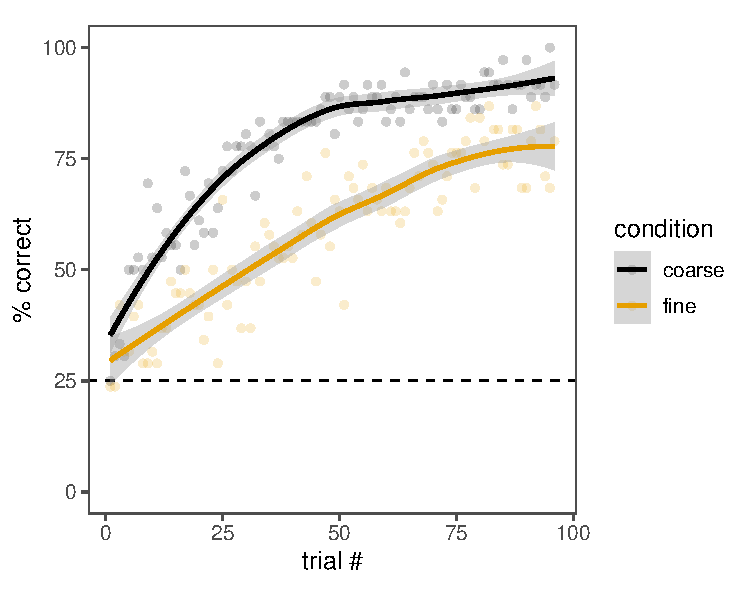
\includegraphics[scale=1]{./figures/sec2_empirical_accuracy.pdf}}
%{\caption{{
%\label{fig:context_accuracy}}}}
%\vspace{-3ex}
%\end{center}
%\end{figure}

\begin{figure}[t]
\begin{center}
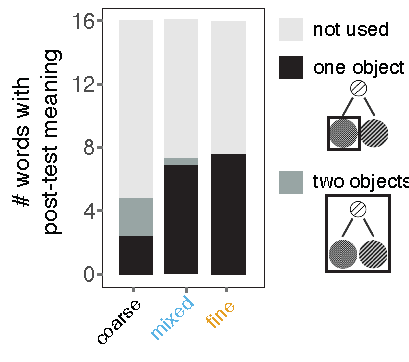
\includegraphics[scale=1]{./figures/Exp2_postTest}
\caption{\emph{Different lexicons emerge in different contexts.} Mean number of words, out of a word bank of 16 words, that human participants reported giving specific meanings (black; applying to 1 object) or abstract meanings (dark grey; applying to 2 objects).}
\label{fig:sec2postTest}
\end{center}
\end{figure}


\subsection{Behavioral results}

\paragraph{Partners successfully learn to communicate}

Although participants in all conditions began with no common basis for label meanings, performing near chance on the first trial (proportion correct $= 0.19$, 95\%~CI~$=~[0.13, 0.27]$), most pairs were nonetheless able to coordinate on a successful communication system over repeated interaction (see Fig.\ \ref{fig:sec2Results}A). 
A mixed-effects logistic regression on listener responses with trial number as a fixed effect, and including by-pair random slopes and intercepts, showed a significant improvement in accuracy overall, $z = 14.4, p < 0.001$. 
Accuracy also differed significantly \emph{across} conditions: adding an additional main effect of condition to our logistic model provided a significantly better fit, $\chi^2(2) = 10.8, p = 0.004$. 
Qualitatively, the \emph{coarse} condition was easiest for participants, the \emph{fine} condition was hardest, and the \emph{mixed} condition was in between.
These effects track the qualitative results of our simulations: our artificial agents were also able to successfully coordinate in both conditions, but did so more easily in the coarse condition than the fine condition. 
%Finally, the (log) response time taken by the speaker to choose an utterance also decreased significantly over the course of the game, $t(126) = -19.7, p < 0.001$, from approximately 20 seconds to only 6 seconds on average, indicating that lexical mappings became increasingly established or accessible.

\begin{figure*}[t]
\begin{center}
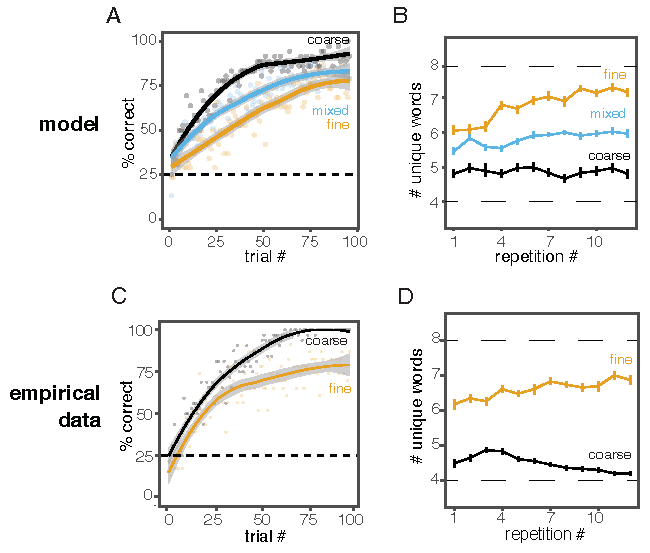
\includegraphics[scale=0.8]{sec2-results-compressed.pdf}
\vspace{1ex}
\caption{\emph{Comparison of simulation results to empirical data}. \ks{are the "model" and "empirical" labels reversed here?} (A) Participants in our behavioral experiment learned to coordinate on a successful communication system, but converged faster in the coarse condition than the fine condition. Each point is the mean proportion of correct responses by listeners; curves are nonparametric fits. (B) The number of unique words used by speakers in each repetition block increased in the fine condition but stayed roughly constant in the coarse condition. (C-D) The same metrics computed on the output of our simulation, qualitatively matching the patterns observed in the empirical data.}
\label{fig:sec2Results}
\end{center}
\end{figure*}
%
%\paragraph{Partners converge on similar conventions}
%
%Another indicator of successful learning is convergence or alignment of lexica between partners within a dyad. 
%Using these estimates of each participant's lexicon, we compute the overlap between partners. 
%For most pairs, partners aligned strongly by the end, with a median post-test overlap of 97.6\% (125 out of 128 entries). 
%Because these matrices were extremely sparse, however, just a a few mismatches could have a large impact on performance. 
%Overall accuracy in the game is strongly correlated with alignment: partners who reported more similar lexica at the end also tended to perform significantly better at the task ($r = 0.77, t(120) = -13.5,~p <0.001$).  
%Despite these broad markers of convergence at the group level, individual performance had a long tail: a subpopulation of 29 games (11\% of coarse games, 18\% of mixed games, and 39\% of fine games) still showed relatively poor performance late in the game (see Fig.~\ref{fig:full_accuracy_grid} in Appendix for full histograms).
%For the subsequent analyses focusing on the content of the lexicon, we exclude games with accuracy below the pre-registered criterion of 75\% on the final quarter of trials to ensure we are examining only the content of lexica that converged.
%\rdh{double-check this. add better motivation if I do this.}

\paragraph{Validating post-test responses}

Before examining post-test responses, we validate their internal consistency.
For each participant, we counted the number of mismatches between the two directions of the lexicon question (e.g.\ if they clicked the word `mawa' when we showed them one of the blue squares, but failed to click that same blue square when we showed `mawa'). 
In general, participants were highly consistent: out of 128 cells in the lexicon matrix (16 words $\times$ 8 objects), the median number of mismatches was 2 (98\% agreement), though the distribution has a long tail (mean $= 7.3$). 
We therefore conservatively take a participant's final lexicon to be the \emph{intersection} of their word-to-object and object-to-word responses for the subsequent analyses.

\paragraph{Contextual pressures shape the lexicon}

We predicted that in contexts regularly requiring speakers to make fine distinctions among objects at subordinate levels of the hierarchy, we would find lexicalization of specific terms for each object (indeed, a one-to-one mapping may be the most obvious solution in a task with only 8 objects). 
Conversely, when no such distinctions were required, we expected participants to adaptively lexicalize more abstract terms.
One coarse signature of this prediction lies in the \emph{efficiency} of the resulting lexicon: lexicalizing abstract terms should require participants to use fewer terms overall.

To test this prediction, we operationalize vocabulary size as the number of words in each participant's reported lexicon in the post-test (i.e.\ the words for which they marked at least one object in the post-test in an internally consistent way). 
We then conducted a mixed-effects models predicting each individual's vocabulary size as a function of dummy-coded condition factors, with random intercepts for each game. 
We found that participants in the \emph{coarse} condition reported significantly smaller, more efficient \ks{more efficient in what sense? not just simpler?} lexica ($m = 4.9$ words) than participants in the \emph{mixed} ($m=7.1, t(110.8)=7.6, p < 0.001$) and \emph{fine} condition ($m = 6.9, t(109.3) = 6.4, p < 0.001$; see Fig.\ \ref{fig:sec2Results}A). 
%At the same time, smaller vocabularies did not lead to poorer coverage over objects: the median number of objects where participants agreed on the same word was 7 out of 8 in the \emph{coarse} condition, compared to 6 in the \emph{mixed} condition and 5.5 in the \emph{fine} condition. 
%Differences across conditions do not reach significance ($p = 0.4, p = 0.09$, respectively), but may reflect the relative sub-populations of participants who did not fully converge. 

How did these lexica emerge over the course of interaction? 
We use the same measure of unique words produced in each repetition block that we used in our simulations. 
We constructed a mixed-effects regression model predicting the effective vocabulary size, including fixed effects of condition and repetition block, and random intercepts and effects of repetition block for each dyad. 
As in the post-test reports, we found an overall main effect of condition, with participants in the fine\ks{coarse?} condition using significantly fewer words across all repetition blocks: $m = 4.9$ in coarse, compared to $m=5.8, t(124)=6.1 \ks{which condition is this?}, p <0.001,$ in mixed $m=6.8, t(124) =11.4, p < 0.001$).
Critically, however, we also found a significant interaction between the coarse and fine conditions \ks{shouldn't this be "between block and condition" or something?}. 
The effective vocabulary size gradually increased over time in the fine condition but remained roughly constant in the coarse condition, $b = 0.12, t = 4.5, p < 0.001$, see Fig. \ref{fig:sec2Results}B.
This interaction, where participants initially attempt to reuse the same terms across targets in the fine condition, is consistent with a gradual differentiation based on communicative need.

Finally, if participants in the \emph{coarse} condition could get away with fewer words in their lexicon, what are the meanings of the words they do have? 
We counted the numbers of `specific' terms (e.g.~words that refer to only one object) and `abstract' \ks{I would avoid "abstract" here to be honest, in favour of "more general" or "less specific" or something} terms (e.g.~words that refer to two objects) in the post-test. 
We found that the likelihood of lexicalizing abstractions differed systematically across conditions.
Participants in the \emph{coarse} condition reported significantly more abstract terms ($m=2.3$) than in the \emph{fine} ($m = 0.24, t(121.2) = 8.5, p < 0.001$) or \emph{mixed} ($m=0.65, t(122.7)= 7.3, p < 0.001$) conditions, where lexicons contained almost exclusively specific terms.
The modal system in the fine condition was exactly eight specific terms with no abstract terms, and the modal system in the coarse condition was exactly four abstract terms (red, blue, striped, spotted) with no specific terms.
However, even in the coarse condition, many individual participants reported a mixture of terms (see Fig.\ \ref{fig:sec2Results}B).


%\paragraph{Model comparison}

%\rdh{TODO: we need to decide which comparisons are most interesting. may need to implement baseline model from other papers (e.g. Steels-style, or Spike et al. implementation?) for a more explicit comparison to models outside our class of Bayesian agents...}

%We compare our model to (1) a simpler case when both agents condition on the same data (i.e. the true target) even after an unsuccessful communication attempt, and (2) ask what happens when we manipulate forgetting parameter, or remove it?
%
%In a non-pragmatic variant of our model, agents use words proportional to their literal meaning and assume their partner is doing the same. 
%In this case, their lexicon converges to a degenerate 1-word (shape) state.
%Because an initial usage is consistent with all levels of abstraction, one of the agents will eventually extend the same word to different object. 
%Then the only way to subsequently accommodate this extension in the interaction history is to rule out more specific meanings. 
%The non-pragmatic agent has no way of knowing that this degenerate solution is confusing to their partner, and will continue to prefer it because it's literally true of every object.

\subsection{Discussion}

There is abundant evidence that languages adapt to the needs of their users, and the context-sensitive emergence of abstractions demonstrated in this section suggests that the driver of this adaptation may lie in the rapid adaptability of agents in individual dyadic interaction. 
By manipulating context statistics in a real-time experiment, we evaluated the extent to which our model captured patterns of context-sensitivity in the behavioral data.

Previous proposals have handled context-sensitivity in different ways.
In some common settings for convention formation, there is no explicit representation of context at all, as in the task known as the ``Naming Game'' where agents coordinate on names for objects in isolation \cite{steels2012experiments,baronchelli2008depth}. 
In other common settings, context is central but held constant throughout interactions, as in Lewis signaling games \cite{lewis_convention:_1969}, where agents use a fixed set of messages to communicate a fixed set of world states \cite{skyrms2010signals,BrunerEtAl14_LewisConventions}.

One of the most sophisticated studies of context in prior work is the Discrimination Game of \citeA{steels2005coordinating}, which examined the joint formation of color categories and color naming conventions.
As in our experiments, contexts were generated randomly on each trial from a large space and stimuli are embedded in a similarity space (with similarity based on Euclidean distance in continuous space rather than taxonomic relations).
Unlike our task, contexts were not systematically manipulated, and the resulting level of abstraction was not evaluated: the only restriction was to ensure that color chips were a fixed minimum distance apart  \cite<see also>[which found that imposing a realistic Just Noticeable Difference function as the minimum distance on communicative contexts leads to human-like color naming systems]{baronchelli2010modeling}. \ks{not clear what point you were making in this paragraph}

In models using simple update rules, the referential context is sometimes accounted for with a \emph{lateral inhibition} heuristic used by both the speaker and listener agents \cite{franke2012bidirectional}.
If communication is successful, the connection strength between the label and object is not only increased, the connection between the label and competing objects (and, similarly, between the object and competing labels) is explicitly \emph{decreased} by a corresponding amount \cite<see also>{steels2005coordinating}.
This lateral inhibition heuristic is functionally similar to our pragmatic reasoning mechanism, in terms of allowing the agent to learn from negative evidence (i.e. the speaker's choice \emph{not} to use a word, or the listener's choice \emph{not} to pick an object). 
Under an inferential framework, however, this property emerges as a natural consequence of well-established Gricean principles of pragmatic reasoning.
Reasoning about a partner's intentions, either while updating beliefs about their lexicon or while selecting an action, naturally instantiates a kind of inductive bias for \emph{mutual exclusivity} \cite{gulordava2020one,ohmerreinforcement,FrankGoodmanTenenbaum09_Wurwur}.

%Our results may help to illuminate the relationship between our concepts and words, which are often treated interchangeably. While our mental taxonomies are adaptive to the natural perceptual structure of the world \cite{MervisRosch81_CategorizationReview} %(Rosch et al, 1976; Mervis \& Rosch ,1981; Murphy \& Smith, 1982), 
%it is far from inevitable that all levels of these conceptual hierarchies become conventionalized as lexical items. There are many perfectly natural concepts that are not represented by distinct words in the English language: for instance, we do not have words for each tree in our yards, or for ad-hoc concepts %like \emph{things to sell at a garage sale} 
%\cite{Barsalou83_AdHocCategories}. Indeed, English speakers are often fascinated by foreign words like the Danish ``hygge'' (a specific notion of coziness) or Scottish ``tartle'' (hesitating when introducing someone because you've forgotten their name) that are difficult to express in English.
%Our results highlight communicative needs to distinguish, in context, as a force behind the choice to lexicalize some fine-grained concepts. 
%A related direction for future work is to explore the relationship between communicative need and \emph{basic-level} structure.
%
%While we showed how abstract words emerge from efficiency even in a task requiring only reference to individual objects, there are other clear functional advantages to having abstract terms in the lexicon. For one, they allow speakers to efficiently refer to large, potentially infinite, sets of things, and make generalizations about categories, e.g.\ ``Dogs bark'' \cite{TesslerGoodman16_Generics}. Future work should explore this as an additional pressure toward abstract, nested nouns.
%Similarly, the option to refer to more specific concepts with compound terms (e.g.~``spotted dog''), which was not available in our experiment, may impact final conventions.
%We expect that labels will become lexicalized when the cost incurred by frequently using a compositional construction exceeds the cost of adding an additional word to the lexicon. 
%Future work should also explore these hypotheses about how lexicalization of nominal terms trades off with compositionality. 
%Our shared lexical conventions are richly structured systems with meanings at multiple levels of abstraction. 
%We are constantly supplementing our existing language with local conventions, as we need them.
